%% $RCSfile: proj_report_outline.tex,v $
%% $Revision: 1.3 $
%% $Date: 2016/06/10 03:41:54 $
%% $Author: kevin $

\documentclass[11pt
              , a4paper
              , oneside
              , openright
              ]{article}


\usepackage{float} % lets you have non-floating floats

\usepackage[usenames, dvipsnames]{color}
\usepackage{url} % for typesetting urls
\usepackage{pdfpages} % for importing the project proposal
\usepackage{listings}  % for code

\lstdefinelanguage{Whiley}{
	keywords={assert, for, while, switch, is, if, case, return,
		else, process, define, as, requires, ensures, where, no,
		all, bool, int, byte, void, real, in, any, null, char,
		string, function, var, method, type, some, reduce, import
	},
	keywordstyle=\color{Plum},
	basicstyle=\ttfamily,
	commentstyle=\rmfamily\itshape\color{gray},
	stringstyle=\small\itshape,
	moredelim=*[s][commentstyle]{/*}{*/}, % allows keyword highlighting inside comments
	morecomment=[l][commentstyle]{//},      % single line comments are set by...
	moredelim=*[s][\color{blue}]{"}{"}, % highlighting print statement
}

%
%  We don't want figures to float so we define
%
\newfloat{fig}{thp}{lof}[section]
\floatname{fig}{Figure}

%% These are standard LaTeX definitions for the document
%%                            
\title{QuickCheck for Whiley Preliminary Report}
\author{Janice Chin}

%% This file can be used for creating a wide range of reports
%%  across various Schools
%%
%% Set up some things, mostly for the front page, for your specific document
%
% Current options are:
% [ecs|msor|sms]          Which school you are in.
%                         (msor option retained for reproducing old data)
% [bschonscomp|mcompsci]  Which degree you are doing
%                          You can also specify any other degree by name
%                          (see below)
% [font|image]            Use a font or an image for the VUW logo
%                          The font option will only work on ECS systems
%
\usepackage[image,ecs]{vuwproject}

% You should specifiy your supervisor here with
     \supervisors{David Pearce and Lindsay Groves}
% use \supervisors if there is more than one supervisor

% Unless you've used the bschonscomp or mcompsci
%  options above use
\otherdegree{Bachelor of Engineering with Honours}
% here to specify degree

% Comment this out if you want the date printed.
\date{}

\begin{document}

% Make the page numbering roman, until after the contents, etc.
\frontmatter

%%%%%%%%%%%%%%%%%%%%%%%%%%%%%%%%%%%%%%%%%%%%%%%%%%%%%%%

%%%%%%%%%%%%%%%%%%%%%%%%%%%%%%%%%%%%%%%%%%%%%%%%%%%%%%%

\begin{abstract}
% TODO abstract
%A short description of the project goes here.

\end{abstract}

%%%%%%%%%%%%%%%%%%%%%%%%%%%%%%%%%%%%%%%%%%%%%%%%%%%%%%%

\maketitle

\tableofcontents

% we want a list of the figures we defined
%\listof{fig}{Figures}

%%%%%%%%%%%%%%%%%%%%%%%%%%%%%%%%%%%%%%%%%%%%%%%%%%%%%%%

\mainmatter

%%%%%%%%%%%%%%%%%%%%%%%%%%%%%%%%%%%%%%%%%%%%%%%%%%%%%%%

% individual chapters included here
\section{Introduction}\label{section:intro}
%This should briefly outline the project and if necessary
%reevaluate the original plan in light of what has been learned in the interim. In particular, any significant deviations in the problem being addressed, or the solution
%being developed should be clearly highlighted and justified.

%The motivation for this project is to ...

% What is Whiley
% What is automatic test case generation

The detection and elimination of bugs is important in software development as it improves the quality and reliability of software.

To help eliminate errors in code, the Whiley programming language was developed to verify code using formal specifications \cite{WhileyLang}.
Ideally, programs written in Whiley should be error free \cite{WhileyLang}.
To achieve this goal, Whiley contains a verifying compiler which employs the use of specifications written by a developer to check for common errors such as accessing an index of an array which is outside its boundaries \cite{WhileyLang}.

Listing \ref{lst:whileyMin} illustrates an example of a Whiley program with a function,  \texttt{min()} which finds the minimum value of two integers. Executing \texttt{min(2, 3)} will return the integer, 2.

\begin{lstlisting}[language=Whiley, tabsize=3, numbers=left,
label={lst:whileyMin}, caption={Whiley program for the min function}]
function min(int x, int y) -> (int r)
ensures r == x ==> x <= y
ensures r == y ==> y <= x:
if x <= y:
	return x
else:
	return y
\end{lstlisting}

Currently, the verifying compiler has limitations when evaluating complex pre- and post-conditions.
For example in Listing \ref{lst:whileySquare}, the post-condition is falsely identified as not holding by the verifying compiler even though the program does meet the post-condition.

\begin{lstlisting}[language=Whiley, tabsize=3, numbers=left,
label={lst:whileySquare}, caption={Whiley program for the square function}]
function square(int x) -> (int r)
	ensures r >= 0:
	return x*x
\end{lstlisting}

Consequently, tests would need to be created to detect if there are further problems within the program. However, writing and running tests can be tedious and costly. Furthermore, it is difficult to write tests for all possible cases and be able to detect all bugs. Instead of manually creating tests, a tool could be created that automatically generates and executes tests on a program such as QuickCheck which was implemented in Haskell by Koen Claessen and John Hughes \cite{QClightweight}.

QuickCheck uses property-based testing and random testing \cite{QClightweight}. Properties defined by the user are used to randomly generate and execute an arbitrary number of tests \cite{QClightweight}. 

Random testing has been widely studied in the literature, leading to the creation of new variants and testing techniques including concolic testing \cite{CUTE}, feedback-directed testing \cite{randoopAll}, \cite{randoopJava} and mutation testing \cite{evoSuite}.

%Other tools have drawn inspiration from QuickCheck with variations in testing techniques including concolic testing \cite{CUTE}, feedback-directed testing \cite{randoopAll}, \cite{randoopJava} and mutation testing \cite{evoSuite}.

This project aims to implement an automated test-case generator for the Whiley programming language, based on the QuickCheck tool. As a result, the automatic test-case generator will improve software quality and increase confidence in unverifiable code. 

Currently, a working implementation of QuickCheck for Whiley has been completed which can generate and execute tests using random and exhaustive test-case generation. 
Constraints applied to integers and array sizes on nominal types have also been implemented to limit the range of integers and size of arrays generated.

% TODO Talk about objectives within the project? Such as the Proposed Solution section of the project proposal

\section{Background Survey}\label{section:background}

%This should discuss any existing solutions to the given problem, and may reference academic papers, books and other sources as appropriate. Care should be taken to identify key differences between these solutions, and that being developed in the project.

There exists a number of different test-case generation tools for different languages such as QuickCheck for Haskell \cite{QClightweight}, Concolic Unit Testing Engine (CUTE) for C \cite{CUTE} and Randoop for Java \cite{randoopJava} and .NET \cite{randoopAll}.

% TODO maybe explain more differences?

QuickCheck for Whiley is specifically created for the Whiley programming language and uses different techniques to generate test data instead of just one technique.

% Something about Whiley, verification and formal specs
\subsection{Whiley}
Whiley is a hybrid imperative and functional programming language developed by David Pearce \cite{WhileyPlatform}. The presentation of Whiley resembles an imperative language like Python whereas the core structure is functional and pure \cite{WhileyPlatform}. 

Functions in Whiley are pure therefore, an input will always result in the same output without any observable side effects \cite{WhileyLang}.
Methods are impure so may have side effects on input parameters or other aspects of the program \cite{WhileyLang}. 
Functions, methods and other compound data types are passed by value meaning they are a copy of the original variable when they are passed in an argument to a function or method \cite{WhileyPlatform}.


A key component in Whiley is the automatic verifying compiler
which is used in conjunction with explicit specifications to verify programs are correct \cite{WhileyPlatform}.
Specifications can be written as pre-conditions (\texttt{requires} clauses) and post-conditions (\texttt{ensures} clauses) in a function or method declaration \cite{WhileyPlatform}.
Specifications can also be written as invariants using \texttt{where} clauses on user defined types (nominal type) or as an invariant on a loop \cite{WhileyPlatform}. 

To be able to execute a Whiley file, it must first be compiled into a WyIL file which is the bytecode form of Whiley in the Whiley Intermediate Language \cite{WhileyPlatform}.
During compilation, the verifying compiler checks all specifications are met and checks for common errors such as division by zero \cite{WhileyPlatform}. Any errors or failed specifications are detected are reported to the developer to fix. Counter examples are also used within Whiley to notify how the specification can fail however, this functionality is limited to examples within a small range.
The WyIL file can then be executed if it verifies successfully or compiled without verification.

\subsection{QuickCheck}
QuickCheck is a tool implemented by Koen Claessen and John Hughes \cite{QClightweight} to test Haskell programs.

To check if a program is correct, QuickCheck uses property-based testing which uses conditions that will always hold true \cite{QClightweight}.
Users define the conditions as Haskell functions in terms of formal specifications to validate functions under test \cite{QClightweight}. 

QuickCheck then generates a large number of test cases automatically using random testing \cite{QClightweight}. 
Input values are randomly generated for each test (within a range) using generators that correspond to the input value's type \cite{QClightweight}. 
QuickCheck contains generators for most of Haskell's predefined types and for functions \cite{QClightweight}. 
User-defined types require the tester to specify their own custom generators with a bounded size if the type is recursive such as a binary tree. \cite{QClightweight}. 

A problem with random testing is the distribution of test data. Ideally, the distribution should adhere to the distribution of actual data which is often uniformly distributed \cite{QClightweight}. 
For example, executing tests for Listing \ref{lst:quickcheckExecute} could be skewed towards test data with short lists. 
The distribution of data is controlled by the tester by creating a custom generator for the data type with weighted frequencies on the methods used to generate the data \cite{QClightweight}.

An example of using QuickCheck would be reversing a list.

Firstly, a property is defined in Listing \ref{lst:quickcheckProperty} where the list \texttt{xs}, should be the same as reversing \texttt{xs} twice.

\begin{lstlisting}[language=haskell, label={lst:quickcheckProperty},
caption={Property for reversing a list in QuickCheck}, captionpos=b, frame = single]
propReverseTwice xs = reverse (reverse xs) == xs
\end{lstlisting}

QuickCheck is then executed by importing the property and passing it into the interpreter as shown in Listing \ref{lst:quickcheckExecute}.

\begin{lstlisting}[label={lst:quickcheckExecute}, caption={Executing tests to check a list is reversed}, captionpos=b,
frame = single]
Main:> quickCheck propReverseTwice
Ok: passed 100 tests.
\end{lstlisting}

A large number of test cases is created where random input values are generated to check the user-defined property holds. QuickCheck reports various test statistics including the number of tests that have passed or failed \cite{QClightweight}.

\subsection{Concolic Unit Testing Engine (CUTE)}
Concolic Unit Testing Engine (CUTE) generates test inputs using a combination of symbolic and concrete execution \cite{CUTE}. 
The aim of CUTE is to provide input values to explore all feasible execution paths of a program and thus achieve high path coverage \cite{CUTE}. CUTE has been applied to C programs \cite{CUTE}.

Random testing may generate inputs with the same behaviour leading to its redundancy \cite{CUTE}. Furthermore, the probability of selecting inputs that will detect errors using random testing is small \cite{CUTE}. 
Therefore, CUTE incrementally generates concrete inputs using symbolic execution to discover feasible paths \cite{CUTE}.

Firstly, CUTE executes the program with arbitrary inputs using concrete and symbolic execution concurrently \cite{CUTE}.
In concrete execution, the program is executed normally with the input values \cite{CUTE}.
At the same time, symbolic execution is run through the same path  \cite{CUTE}. 
Using the symbolic variables, constraints from branching expressions are discovered and stored \cite{CUTE}.
The last constraint applied is negated so that the next test run will explore a different feasible path \cite{CUTE}. 
The constraint is solved to limit and determine the possible inputs to execute in the next test \cite{CUTE}.

For example, we execute Listing \ref{lst:cuteExample} and create the random values \texttt{x = y = 1}. 
In concrete execution, \texttt{z} is set to 1 whereas in symbolic execution, \texttt{z} is set to \texttt{x * y}.
At line 2, \texttt{x != 2} so the condition fails. 
As the program went through one path where \texttt{x != 2}, the condition is then negated and solved so the next test goes through a different path by setting \texttt{x} to 2 and y to 1. 
The test will then fail at line 4 as \texttt{x >=z}. Therefore, CUTE will then find values that solve the constraints \texttt{x == 2} and \texttt{x < z} such as \texttt{x = 2} and \texttt{y = 2}. 
Running this test will then exhibit the error on line 5. 


%Firstly, CUTE executes the program with arbitrary inputs using concrete and symbolic execution concurrently \cite{CUTE}.
%For example, we execute Listing \ref{lst:cuteExample} and create the random values \texttt{x = y = 1}. 
%In concrete execution, the program is executed normally with the input values \cite{CUTE}.
%At the same time, symbolic execution is run through the same path  \cite{CUTE}. 
%In concrete execution, \texttt{z} is set to 1 whereas in symbolic execution, \texttt{z} is set to \texttt{x * y}.
%Using the symbolic variables, constraints from branching expressions are discovered and stored \cite{CUTE}. At line 2 in the example, \texttt{x != 2} so the condition fails. 
%The last constraint applied is negated so that the next test run will explore a different feasible path \cite{CUTE}. 
%The constraint is solved to limit and determine the possible inputs to execute in the next test \cite{CUTE}.
%As the test failed the last condition as \texttt{x != 2}, the condition is negated and solved so in the next test, \texttt{x} is set 2 and y remains set to 1. The test will fail at line 4 as \texttt{x >=z}. Therefore, CUTE will then find values that solve the constraints \texttt{x == 2} and \texttt{x < z} such as \texttt{x = 2} and \texttt{ y = 2}. Running this test will then exhibit the error on line 5. 

\begin{lstlisting}[language=C, tabsize=3, numbers=left,
label={lst:cuteExample}, caption={Example C program}]
void foo(int x, int y) {
	int z = x * y;
	if(x == 2){
		if(x < z){
			ERROR;
		}
	}
}
\end{lstlisting}

\subsection{Randoop}
Randoop which stands for random tester for object-oriented programs, generates unit tests using feedback-directed random test generation \cite{randoopAll}, \cite{randoopJava}. Method sequences from previous tests are used to help generate subsequent tests \cite{randoopAll}, \cite{randoopJava}.
As a result, a test suite is outputted with successful and unsuccessful tests \cite{randoopAll}, \cite{randoopJava}.

Randoop tests classes by executing a sequence of methods as a test \cite{randoopJava}. Method sequences are created incrementally by randomly selecting method calls and using arguments from previous sequences \cite{randoopJava}.
The sequence is then executed and checked against contracts \cite{randoopAll}.
Contracts are built into Randoop or optionally defined by the user \cite{randoopAll}.
If a sequence breaks a contract, then the test is outputted as a contract-violating test \cite{randoopAll}. If sequence was successful, then the test is outputted as a regression test \cite{randoopAll}.
Successful sequences that are not redundant and can be extended are used in subsequent tests \cite{randoopAll}.


For example, executing Randoop on the Java program in Listing \ref{lst:randoopJavaProg} will produce several tests based on different method sequences.
One successful list of method sequences could be Listing \ref{lst:randoopSuccess},  which can be re-used in subsequent sequences. It is outputted into a regression test as shown in Listing \ref{lst:randoopSuccessTest}.
By extending the method sequences, another list of method sequences is created such as Listing \ref{lst:randoopError}.
This list of method sequences throws an error as the \texttt{equals()} method is incorrect as \texttt{a1} is not equal to \texttt{b1} and thus, is a contract-violating test that will be outputted.

\begin{lstlisting}[language=Java, tabsize=3, numbers=left,
label={lst:randoopJavaProg}, caption={Example Java class}]
public class A {
	public A(){ }
		
	@Override
	public boolean equals(Object obj){
		return true;
	}
}

public class B{
	public B(){ }
}
\end{lstlisting}

\begin{lstlisting}[language=Java, tabsize=3, numbers=left,
label={lst:randoopSuccess}, caption={Successful method sequence for testing Listing \ref{lst:randoopJavaProg}}]
A a1 = new A();
a1.equals(a1);
\end{lstlisting}

\begin{lstlisting}[language=Java, tabsize=3, numbers=left,
label={lst:randoopSuccessTest}, caption={Test output for the successful method sequence in Listing \ref{lst:randoopSuccess}}]
@Test
public void test1() {
	A a1 = new A();
	assertTrue(a1.equals(a1));
}
\end{lstlisting}

\begin{lstlisting}[language=Java, tabsize=3, numbers=left,
label={lst:randoopError}, caption={Contract violating method sequence for testing Listing \ref{lst:randoopJavaProg}}]
A a1 = new A();
a1.equals(a1);
B b1 = new B();
a1.equals(b1);
\end{lstlisting}

%A commercial version of QuickCheck in Erlang called Quviq QuickCheck is co-founded by one of the original developers, John Hughes and is an extension of the original QuickCheck for Haskell \cite{QCFunProfit}.

% JCrasher?
% EvoSuite?
% Quviq QuickCheck
\section{Work Completed}\label{section:work}

%This should discuss what progress has been made on designing, implementing and evaluating the artifact. Care must be taken to ensure that any discussion of technical points are clearly explained, with diagrams being used where appropriate.
%In many cases, the evaluation proper will not yet have begun. However, it is important to demonstrate that sufficient thought has been given to the evaluation.

% Consideration of test generation techniques used
% Trade off => Performance vs accuracy?
% Needed to create test cases that adhered to the pre-conditon

An implementation of the tool has been created with generation of core and more complex data types. 
The tool has also been extended to use integer range analysis to constrain input values generated for better performance. 
Unit tests have also been written to check the tool generates the values expected.

The tool can be executed via the command line with several arguments. To use the tool, a user must pass in the path of a WyIL file and specify the test case generation technique to use, number of tests they wish to generate and ranges for generating integer values. Ranges are used to limit the integers generated between an inclusive, minimum number and an exclusive, upper number.

Whiley's interpreter is used to validate inputs and outputs from tests. Valid inputs are based on verifying pre-conditions and constraints on the input type used. Only valid inputs are used in tests. A successful test is checked by verifying outputs with the function's post-conditions and constraints on the outputs' type.

% These invalid inputs should be discarded and replaced by generating new input data.

An example of using the tool is to test the file \texttt{abs.wyil} which contains the following code in Listing \ref{lst:whileyAbs}.
To execute the tool, we run in the command line: 
\begin{verbatim}
java QuickCheck abs.wyil exhaustive 10 -5 5
\end{verbatim}

This tells QuickCheck for Whiley to generate 10 tests using exhaustive test case generation with an integer range between -5 and 5. 
When the tool is executed, it outputs several statistics for the user as shown in Listing \ref{lst:whileyQCResults} including the number and percentage of tests that passed and failed and the inputs that failed.

\begin{lstlisting}[language=Whiley, tabsize=3, numbers=left,
label={lst:whileyAbs}, caption={Whiley program for an incorrect implementation of the abs function},
captionpos=b]
function abs(int x) -> (int r)
ensures r >= 0
ensures r == x || r == -x:
	return x
\end{lstlisting}

\begin{lstlisting}[label={lst:whileyQCResults},
caption={Results of executing the tool on Listing \ref{lst:whileyAbs}},
captionpos=b, frame=single ]
Failed Input: [-5] Output: [-5]
Failed Input: [-4] Output: [-4]
Failed Input: [-3] Output: [-3]
Failed Input: [-2] Output: [-2]
Failed Input: [-1] Output: [-1]
Failed: 5 passed (50.00 %), 5 failed (50.00 %), ran 10 tests
\end{lstlisting}

\subsection{Test Case Generation Techniques}

QuickCheck for Whiley currently employs random test case and exhaustive test case generation to generate test cases. A test case in QuickCheck for Whiley tests one function or method using a set of generated input values.

\subsubsection{Random Test Case Generation}

A fixed number of tests determined by the user is randomly generated.
To randomly generate a value for a particular type, the type is quantified into a numeric range of valid values. 
A random integer value is pseudorandomly created from a seed and used to select a value out of the range of valid values.
A problem encountered using random generation is that previous inputs are not considered which may lead to the same inputs being generated.
Knuth's Algorithm S from \cite{artProgv2} was considered to generate unique inputs to solve this problem but has not been implemented yet.

\subsubsection{Exhaustive Test Case Generation}
A fixed number of tests determined by the user are exhaustively generated. Ranges are used to limit integers and the size of arrays during generation so that a feasible number of values are generated. 
Exhaustive test generation uses the \texttt{size()}, \texttt{exceedCount()}, and \texttt{resetCount()} methods to generate the correct value as shown in Figure \ref{fig:qc-generators}.
The number of unique values that can be generated is determined by using the \texttt{size()} method.
\texttt{exceedCount()} is used to check if the number of tests exceed the number of unique values. If this occurs, then \texttt{resetCount()} is called so that the tool will cycle around and generate inputs exhaustively from the starting value. 
Integers are generated by starting from the lower limit. Arrays are generated by starting from the smallest possible array size, which is usually an empty array. 

\subsection{Data types generated}
Different generators are created for the different types defined in Whiley. Each generator generates a value for their corresponding type.
Figure \ref{fig:qc-generators} illustrates the structure of the generators used.
 
\begin{figure}
	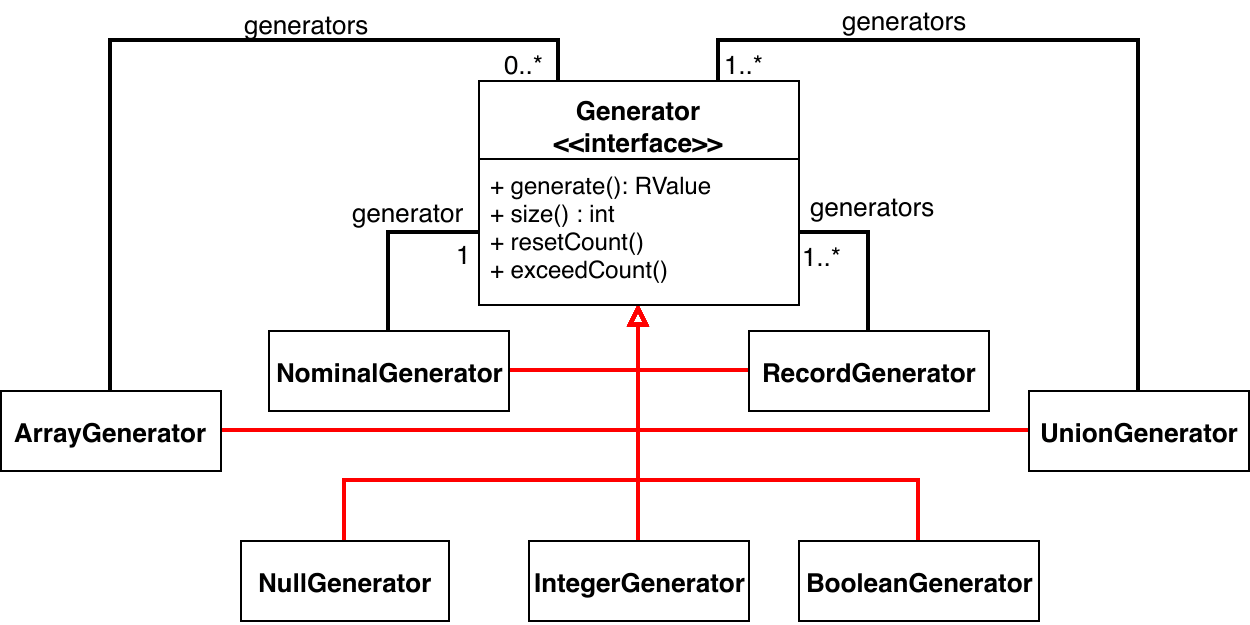
\includegraphics[width=\textwidth]{qc-generators}
	\caption{Class diagram of Generators in QuickCheck for Whiley}
	\label{fig:qc-generators}
	\centering
\end{figure}

\begin{description}
	\item[Null] Generate a \texttt{null} value.
	\item[Boolean] Generates a Boolean which is either \texttt{true} or \texttt{false}.
	\item[Integer] Generates an integer between a bounded range. This range may be modified based on constraints applied to the integer.
	\item[Array] Generates an array with a specific element type between a bounded size range.
	The size of arrays is currently limited to a maximum size of three elements due to the performance cost of generating larger arrays.
	\item[Nominal] A nominal represents a user-defined type by redefining a type with a different name \cite{WhileyLang}.
	Therefore, a generator for a nominal wraps a generator for a different type to generate a value. 
	A nominal can also have a type constraint applied to it \cite{WhileyLang}.
	\item[Record] "A record type describes the set of all compound values made from one or more fields, each of which has a unique name and a corresponding type \cite{WhileyLang}."
	A closed record contains a fixed number of fields whereas an open record can have any number of fields with different types \cite{WhileyLang}.
	A closed record is generated by generating values that correspond to each field. Generators corresponding to each field is required as each field may have different types. 
	Generation for open records has not been implemented as there can be an arbitrary number of fields added to a record. 
	This could be a future extension to the tool.
	\item[Union] A union is made up of multiple types where the union's value corresponds to any one of the types declared. For example, the type \texttt{bool|int} can hold either a boolean or an integer value. 
	A union is generated by generating a value from one of the declared types. A generator corresponding to each type is required.
	Recursive unions such as \texttt{type list is \{int value, list next\} | null} have not been implemented as they can recursively generate themselves indefinitely. 
	A solution to this would be to limit the number of recursive values generated.
	% Talk about fairness in union generation

	Values for the union type could be skewed towards generating values for only one type. It was important that the different types for each union are generated fairly. Therefore, the union generator was implemented so that a value from a different type would be generated each time by iterating through the generators within the union generator.

\end{description}

\subsection{Integer Range Analysis}

Generating and checking for invalid inputs is costly in terms of performance. 
Therefore, it would be beneficial to reduce the number of invalid inputs generated to improve the performance of the tool.
One method to remove invalid inputs for integers is to shrink the ranges used during generation, thus preventing the generation of invalid inputs.

For example, a nominal type is defined, \texttt{type nat is (int x) where x \textgreater= 0} and the tool is executed for an integer range between -5 and 5. An integer generator for this input will only generate numbers between 0 and 5; removing the need to generate then discard invalid inputs which are numbers below 0.

This is implemented by evaluating the constraints within a nominal type to discover integer range generated from the constraint.
Existing code from \cite{whileyIntegerRangeCode} from the work in \cite{whileyIntegerRange} was used to create the integer ranges.
The discovered integer range is passed down in the nominal generator until it reaches the relevant integer or array generator where it is intersected with an existing range.
If the ranges are invalid, i.e. the lower range is greater than the upper range then an error is thrown.

A number of issues were encountered when evaluating constraints.
Constraints with multiple parameters such as \texttt{x < y}, cannot be evaluated as there are no constant values to limit the parameters. 
Another constraint that is difficult to evaluate is when a constant has additional terms for example, \texttt{x - 2 > 10}. 
This requires reversing operations so that all constants are evaluated on one side of the constraint (i.e. \texttt{x > 10 + 2}). 
Therefore, only constraints of the following format is evaluated: \texttt{x op c} where \texttt{x} is the named variable in the nominal type, \texttt{op} is an operator out of the set \{\textgreater, \textless, \textgreater=, \textless=, \&\&, $||$, ==\} and \texttt{c} is a constant number. 
Currently, integer ranges are only applied to constraints on nominal types. 
However, this could be extended to arguments using a function or method's precondition.

\subsection{Evaluating the tool}
\label{subsec:toolEval}
The tool has been evaluated by executing a variety of tests notably, the test suite for the Whiley Compiler containing tests for valid and invalid inputs and outputs \cite{whileyCompilerTests}. 
Valid tests should always pass for valid inputs whereas invalid tests should always fail for some valid input. 
A successful implementation of the tool should pass all tests.

To evaluate the Whiley Compiler test suite, the tool is executed twice using exhaustive test generation for each test to generate a feasible number of combinations. 
The first execution is with a negative integer range between -5 (inclusive) and 0 (exclusive) whereas the second execution is with a positive integer range between 0 (inclusive) and 5 (exclusive).
Currently, the tool passes 80.69\% (4 s.f) (422 out of 523 tests) of the valid tests taking roughly 50 seconds to execute and passes 93.49\% (4 s.f.) (316 out of 338 tests) of the invalid tests taking roughly 15 seconds to execute \cite{qcWhileyStatistics}. 
Some of the tests may falsely pass by the tool due to the small domain of integer ranges used. 
For example, a test could have type constraint on a nominal type where the wrapped integer is greater than 10 which is outside the ranges tested. 
Therefore, some tweaking will be required to determine a suitable integer range across all tests.

% Talk about how the tool is run
% Talk about evaluating the tool using the Whiley valid and invalid tests
% How to evaluate the tool
\section{Future Plan}\label{section:future}

%This should highlight the main components which remain to be done, and provide a proposed time-line in which this will happen. In putting together a time line, students must take into account upcoming examinations, coursework deadlines
%and other disruptions.

A working implementation has been completed halfway through the project. However, there are still several components that need to be completed.
A timeline of these components is shown in Table \ref{table:timeline}

\begin{table}[H]
	  \centering
\begin{tabular}{ |p{10cm}|p{2cm}|p{2cm}|p{2cm}| }
\hline
\textbf{Output} & \textbf{Estimated Time} & \textbf{Start Date} & \textbf{Complete by}\\
\hline
Optimise functions/method calls when testing a specific function/method to improve the performance of the tool. & 3 weeks & 11/6/18 & 2/7/18 (Exam period) \\
\hline
Produce slides for presentation of preliminary report & 1 week & 2/7/18 & 9/7/18 (Break)\\
\hline
Add mutation testing by mutating Whiley files and comparing results from the mutated files with the original file. & 3 weeks & 9/7/18 & 30/7/18 (Week 3)\\
\hline
Produce draft of final report & 6 weeks & 30/7/18 & 15/9/18 (Week 7)\\
\hline
Evaluate the automatic test-case generator using the different test-case generation techniques against a test suite. & 3 weeks & 15/9/18 & 5/10/18 (Week 10) \\
\hline
Finalise final report & 2 weeks & 6/10/18 & 21/10/18 (Week 12) \\
\hline
Prepare slides for final presentation & 3 weeks & 22/10/18 & 16/11/18 (Exam period)\\
\hline
\end{tabular}

\caption{Timeline}
\label{table:timeline}

\end{table}

% Generation - byte, reference, recursive types? 
\section{Request for Feedback}\label{section:feedback}

%This should highlight any difficulties currently faced, and
%make specific requests for guidance from the examination committee. For example, a student may be unsure how best to evaluate their artifact, and would appreciate
%suggestions for alternative methods.


%%%%%%%%%%%%%%%%%%%%%%%%%%%%%%%%%%%%%%%%%%%%%%%%%%%%%%%

\backmatter

%%%%%%%%%%%%%%%%%%%%%%%%%%%%%%%%%%%%%%%%%%%%%%%%%%%%%%%


\bibliographystyle{ieeetr}
%\bibliographystyle{acm}
\bibliography{sample}

\appendix

\section{Project Proposal}\label{section:proposal}

\includepdf[pages=-]{"../Project Proposal/Project Proposal".pdf}

\end{document}
